\documentclass{article} \usepackage{amsmath} \usepackage{amssymb} \usepackage{amsthm} \usepackage[margin=0.2in]{geometry} \usepackage{hyperref} \usepackage{physics} \usepackage{tikz} \usepackage{mathtools} \mathtoolsset{showonlyrefs} \theoremstyle{definition} \newtheorem{theorem}{Theorem}[section] \newtheorem{corollary}{Corollary}[theorem] \newtheorem{lemma}[theorem]{Lemma} \newtheorem{definition}{Definition}[section] \author{Connor Duncan} \date{\today}
\title{Physics-105-Lecture-Notes-03-07-2019}
\begin{document}
\maketitle\tableofcontents
\noindent\abstract{A single PDF with all lectures in a single document can be downloaded at \url{https://www.dropbox.com/sh/8sqzvxghvbjifco/AAC9LoSRnsRQDp7pYedgWpQMa?dl=0}. The password is 'analytic.mech.dsp'.
 This file was automatically generated using a script, so there might be some errors. If there are, you can contact me at \url{mailto:ctdunc@berkeley.edu}.}
\subsection{Recall} Recall that we can write the hamiltonian in terms of the lagrangian as $H=p\dot q-\mathcal L(q,\dot q(q,p),t)$, with $p=\pdv{\mathcal L}{\dot q}$, called the canonical momentum. Using the euler lagrange equation, we derived \begin{align} \dot q=\pdv{H}{p}\\ \dot p=-\pdv{H}{q}\\ \pdv{H}{t}=-\pdv{\mathcal L}{t} \end{align} which are hamiltons equations of motions, which are \emph{all first order equations} which is convenient!. \subsection{Stationary Phase Derivation} Recall \begin{equation} S=\int_{t_1}^{t_2}\mathcal{L}dt \end{equation} + we used to minimize this bad boy. Now, let \begin{equation} S=\int_{t_1}^{t_2}\left(p\dot q-H\right)dt \end{equation} Now, using calculus of variations, let's replace $q\rightarrow q+\epsilon\eta, p\rightarrow p+\epsilon\chi$, with $\eta(t_1)=\chi(t_1)=\eta(t_2)=\chi(t_2)=0$, giving \begin{equation} S=\int_{t_1}^{t_2}\left(\left(p+\epsilon\chi\right)\left(\dot q+\epsilon\dot\eta\right)-H(q+\epsilon\eta,p+\epsilon\chi,t)\right)dt \end{equation} which gives \begin{align} \delta S=\epsilon\int\left(p\dot\eta+\chi\dot q-\pdv{H}{q}\eta-\pdv{H}{p}\chi_)+\mathcal O(\epsilon^2)\right)dt\\ =\epsilon\int_{t_1}^{t_2}dt\left((\dot q-\pdv{H}{p})\chi-(\dot p+\pdv{H}{q})\eta\right) \end{align} In order for this to go to zero, we must have \begin{align} \dot q-\pdv{H}{p}=0 && \dot p+\pdv{H}{q}=0 \end{align} which derives the equations of motion! \subsection{Ray Tracing} We can analogize this to ray tracing (which if I had to guess won't be on the exam). Basically, we can use energy to follow paths through ray tracing. \section{Canonical Transformation} \subsection{Laying the Groundwork} \subsubsection{Legendre Transformations} Consider some function \begin{center} \begin{tikzpicture} \draw[->] (0,-.2)--(0,1) node[anchor=south]{$y$};\draw[->](-.2,0)--(1,0) node[anchor=west]{$x$}; \draw[scale=0.5,domain=-1:1,smooth,variable=\x,blue] plot ({\x},{2.71^\x}); \end{tikzpicture} \begin{tikzpicture} \draw[->] (0,-.2)--(0,1) node[anchor=south]{$n$};\draw[->](-.2,0)--(1,0) node[anchor=west]{$m$}; \draw[scale=0.5,domain=-0:1,smooth,variable=\x,blue] plot ({\x},{-(\x+1)*(\x+1)/2+2}); \end{tikzpicture} \end{center} We're transforming to tangency space, so at some point we have (in two variables) \begin{align} f(x,y) \end{align} so that \begin{align} f(x,y)\rightarrow df=\pdv{f}{x}dx+\pdv{f}{y}dy \end{align} and write \begin{align} u=\pdv{f}{x}\\ v=\pdv{f}{y} \end{align} so we want to transform from $(x,y)\rightarrow (v,y)$. write that \begin{align} g=f-ux\\ dg=df-udx-xdu=(udx+vdy)-udx-xdu\\ dg=vdy-xdu=\pdv{g}{y}dy+\pdv{g}{v}du\\ \end{align} which, post legendre-transform gives \begin{align} v=\pdv{g}{y} && x=-\pdv{g}{u} \end{align} which kind of looks like the hamiltonian! \subsubsection{Hamiltonian$\Leftrightarrow$Legendre Transformation} \begin{equation} (q,\dot q,t)\rightarrow (q,p,t) \end{equation} We can show this by saying that (letting lagrangian correspond now to $L$ instead of $\mathcal L$), \begin{align} dL=\pdv{L}{q}dq+\pdv{L}{\dot q}d\dot q+\pdv{L}{t}dt\\ p=\pdv{L}{\dot q}\\ \Downarrow\\ dL=\dot pdq+p\dot q+\pdv{L}{t}dt\\ \dv{}{t}\left(\pdv{L}{\dot q}\right)=\pdv{L}{q}=\dot p \end{align} This then becomes \begin{align} dH=\dot qdp+pd\dot q-\left(\dot pdq+pd\dot q+\dv{L}{t}dt\right)\\ =\dot dp-\dot pdq-\pdv{L}{t}dt=\pdv{H}{q}dq+\pdv{H}{p}dp+\pdv{H}{t}dt \end{align} which, equating term by term gives hamiltons equations of motion, under a legendre transformation. \subsubsection{Steps for Solving Hamiltonian Dynamics} \begin{enumerate} \item Choose coordinates $q$, construct $\mathcal L$. \item Get Canonical Momentum $p=\pdv{\mathcal L}{q}$. \item Find the hamiltonian $H(q,\dot q,p,t)=\dot qp-\mathcal L(q,\dot q,t)$. \item invert $p=\pdv{\mathcal L}{q}$ to get $\dot q(q,p,t)$ \item Eliminate $\dot q$ from $H\rightarrow H(q,p,t)$. \end{enumerate} \subsubsection{Particle in Gravity} \begin{align} L=T-V=\frac{1}{2}m\left(\dot x^2+\dot y ^2+\dot z^2\right)-mgz \end{align} and \begin{align} p_x=m\dot x && p_y=m\dot y && p_z=m\dot z \end{align} which gives \begin{align} H=\frac{1}{m}\left(p_x^2+p_y^2+p_z^2\right)-\left(\frac{1}{2}m\left(\dot x^2+\dot y ^2+\dot z^2\right)-mgz\right) \end{align} Under the Legendre transformation, we get that \begin{equation} H(q,p)=\frac{1}{2m}\left(p_x^2+p_y^2+p_z^2\right)+mgz \end{equation} which gives that $\dv{x}{t}=\pdv{H}{p_x}=\frac{p_x}{m}$, so the whole thing just comes out to be that \begin{equation} \dot p_z=p\pdv{H}{q}=-mg \end{equation} \subsubsection{Liouville Theorem} Let's take phase space \begin{center} 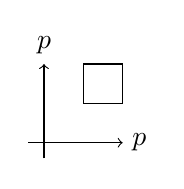
\begin{tikzpicture} \draw[->] (0,-.2)--(0,1) node[anchor=south]{$p$};\draw[->](-.2,0)--(1,0) node[anchor=west]{$p$}; \draw (0.5,0.5) rectangle (1,1); \end{tikzpicture} \end{center} Let some box in $p,q$ phase space with side lengths $\Delta p,\Delta q$. Let $\rho\equiv$density of points in $q,p$, or phase space density. How many particles cross the left face of the box (closest the $p$ axis, orthogonal to $q$) in time $dt$? We write $dn=\rho\Delta q\Delta p$, with $\Delta q=\dv{q}{t}dt=qdt$ With indices, we can say that \begin{equation} dN_2=\left.\rho\dot q\right|_{q+\Delta q}dt\Delta p \end{equation} which gives \begin{align} dN_{12}=dN_1-dN_2=\left(\left.\rho\dot q\right|_{q}-\left.\rho\dot q\right|_{q+\delta q}\right)dt\Delta p \end{align} we can do the same thing along the $p$ axis as well. Interpreting this, we can think of particles entering and exiting the box. If more go in than come out, then we have some weird shenanigans happening. We can write the $p,q$ equations as derived above as a single differential equation \begin{equation} \pdv{\rho}{t}+\pdv{}{q}\left(\rho\dot q\right)+\pdv{}{p}\left(\rho \dot p\right)=0 \end{equation} which is a continuity equation for phase space. Simplifies to \begin{equation} \left(-\pdv{}{q}\left(\rho\dot q\right)-\pdv{}{p}\left(\rho\dot p\right)\right)dt\Delta q\Delta p=\pdv{\rho}{t}\Delta t\Delta q\Delta p \end{equation} where the left side is the particles entering, exiting the box in each direction, and the right side is the change in density. Wrriten in hamiltonian mechanics, the liouville theorem is expressed as \begin{equation} \pdv{p}{t}+\pdv{H}{p}\pdv{\rho}{q}-\pdv{H}{q}\pdv{\rho}{p}=0 \end{equation} watch out for the Poisson Brachet. It'll come up later.
\end{document}
